
\begin{figure*}[t]
  \centering
  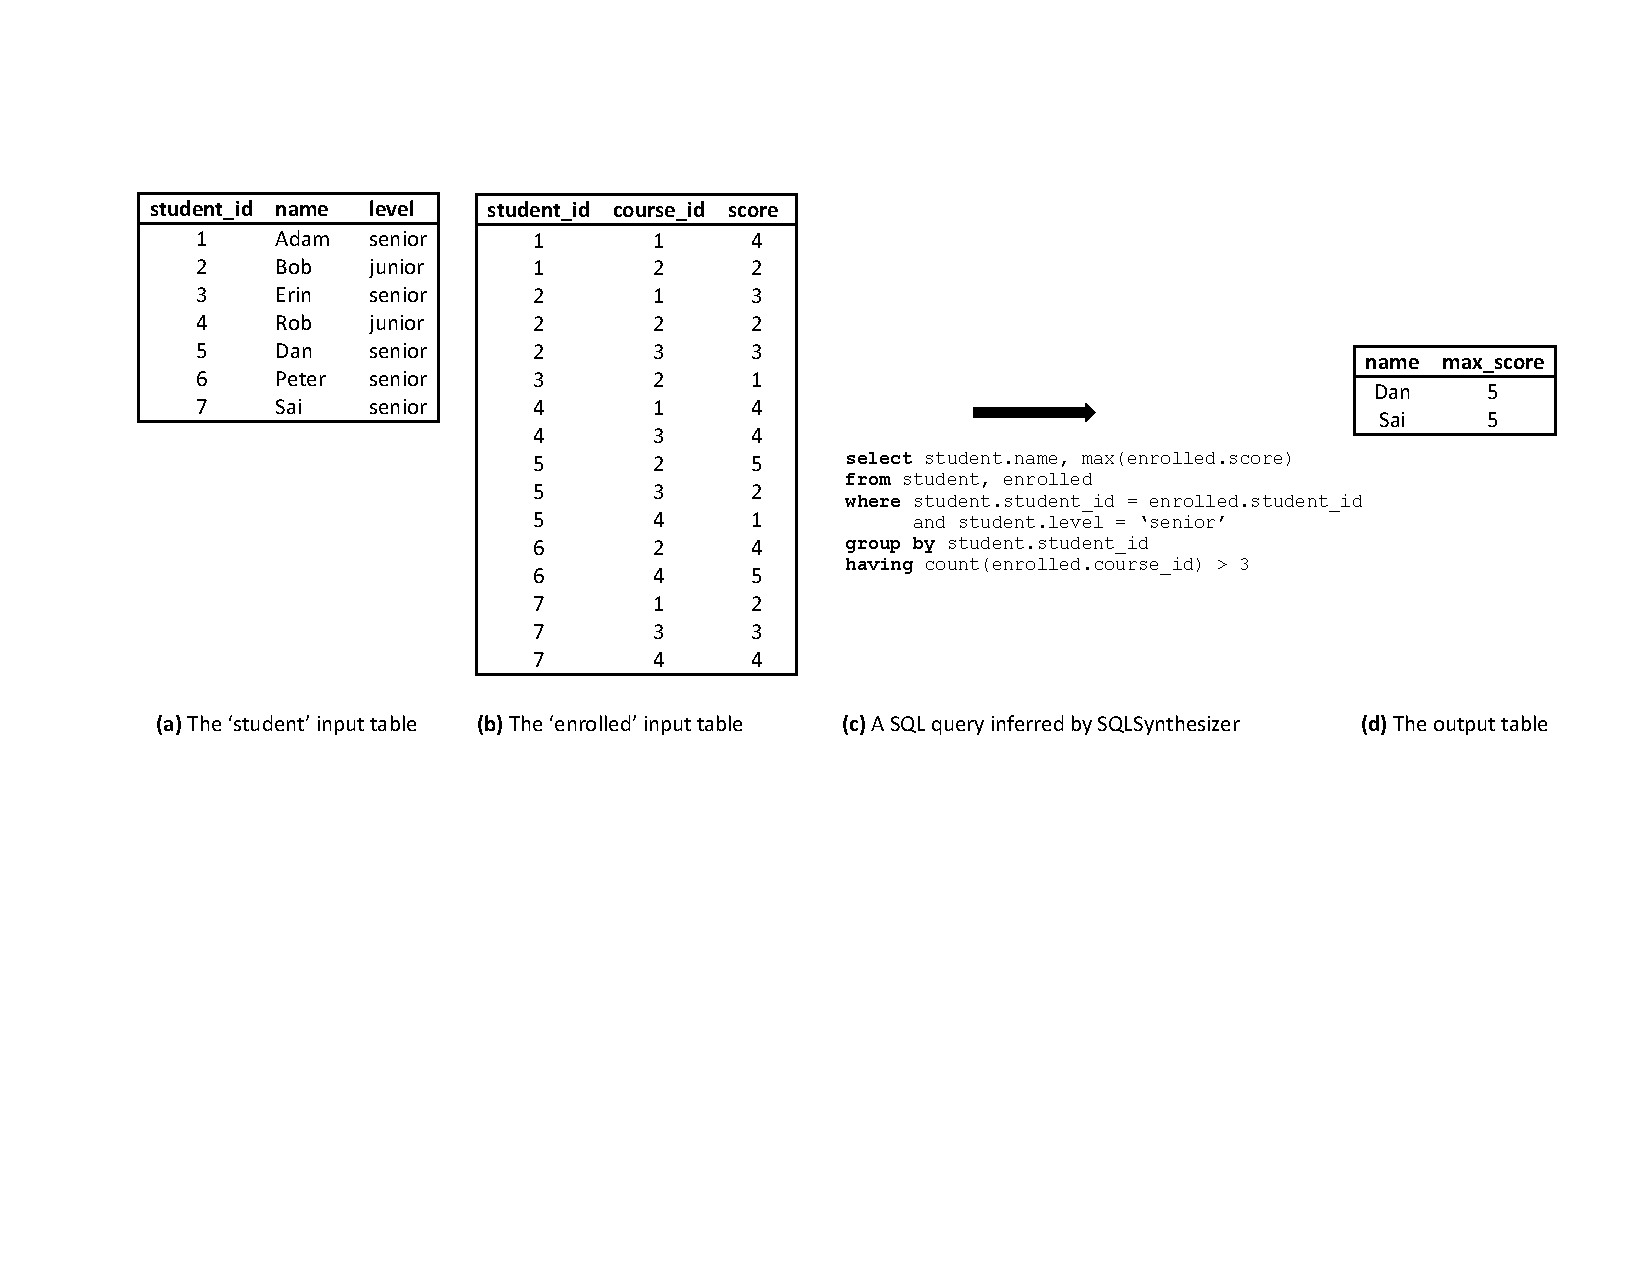
\includegraphics[scale=0.70]{motivating}
  \vspace*{-1.0ex}\caption {{\label{fig:motivating}
  Example input-output tables and the SQL query sythensized by
  \ourtool. In this example, users provide \ourtool with
  two input tables (shown in (a)) and an output table (shown in (c));
  \ourtool automatically infers a SQL query (shown in (b)) that
  transforms the two input tables into the output table.
}}
\end{figure*}

\section{Illustrating Example}
\label{sec:example}

We use the example in Figure~\ref{fig:motivating} (described below)
to illustrate the use of \ourtool. This example is
adapted from a SQL exercise from a classic
database textbook~\cite{cowbook} (Chapter 5, Exercise 1),
and has been simplified for illustration purpose.

\begin{quote}
\textit{Find the name and the maximum course score of all senior student
who are enrolled in more than 2 courses.}
\footnote{
Shown in Figure~\ref{fig:motivating}, the \CodeIn{student} table
contains three columns: \CodeIn{student\_id}, \CodeIn{name},
and \CodeIn{level}. Table \CodeIn{enrolled} contains
three columns: \CodeIn{student\_id}, \CodeIn{course\_id},
and \CodeIn{score}.
%a \CodeIn{enrolled} table having three columns:
%\CodeIn{student\_id}, \CodeIn{course\_id}, and \CodeIn{score}.
}
\end{quote}


The desirable SQL query, as \ourtool inferred in
Figure~\ref{fig:motivating}(b), first joins the
\CodeIn{student} and \CodeIn{enrolled} tables,
then groups by the joined table by the \CodeIn{student\_id}
column and selects students enrolled in more
than 3 courses (the \CodeIn{having} statement).
After that, this query further selects students
whose level is \CodeIn{senior} and uses the \CodeIn{max}
aggregator function to compute the maximum course score.


Despite the simplicity of the problem description,
to write the desirable SQL query, end-users must manually
connect their understanding of the task
with specific SQL language features that can be used to
fullfil the task. Such a process can be non-trivial
for novice users.  In addition, to the best of our knowledge,
none of the existing SQL synthesis techniques~\cite{Zloof:1975,
Tran:2009, DasSarma:2010, abs-1208-2013}
can help uers write the above query\todo{right place?}

As illustrate in Figure~\ref{fig:motivating}, an alternative
approach to write this query is to provide \ourtool
with some representative input-output examples; and
let \ourtool automatically automatically infer the query.
\todo{transition}


